% !TEX program = xelatex
\documentclass[aspectratio=169]{beamer}
\usepackage[italian]{babel}
\usepackage{animate}
\usepackage{mathtools,color}
\usepackage[makeroom]{cancel}
\usepackage{multicol}
\usepackage{mathrsfs}
\usepackage{tikz}
\usepackage{fontspec}
\usepackage{booktabs}
%\usepackage{bbold}
\usepackage[bold-style=ISO]{unicode-math}
\usepackage{tikz-3dplot}

\setmainfont{XITS}
\setmathfont{XITS Math}
\setmathfont[range={\mathcal,\mathbfcal},StylisticSet=1]{XITS Math}


\usetikzlibrary{fadings}
\usetikzlibrary{patterns}
\usetikzlibrary{shadows.blur}
\usetikzlibrary{shapes}
\usetikzlibrary{matrix,backgrounds,3d,positioning}


\usetheme{Rochester}

\definecolor{codegreen}{rgb}{0,0.6,0}
\definecolor{codegray}{rgb}{0.5,0.5,0.5}
\definecolor{codepurple}{rgb}{0.58,0,0.82}
\definecolor{backcolour}{rgb}{0.95,0.95,0.92}
 
\newfontfamily\Lato[Ligatures=TeX]{Lato}

\usefonttheme{professionalfonts}

\setsansfont{Lato}[
  UprightFont=*-Light,
  ItalicFont=*-LightItalic,
  BoldFont=*-Regular,
  BoldItalicFont=*-Italic
]

\renewcommand{\CancelColor}{\color{red}}



\uselanguage{Italian}
\languagepath{Italian}



\title{Transfer learning per selezionare gli informative-frame in una laringoscopia usando learned features}
\subtitle{Tesi di Laurea in Ingegneria Informatica}
\date{A.A. 2020/2021}
\author{Laureando: Bortolin Simone\\Relatore: Nanni Loris} 
\begin{document}

\begin{frame}
    \maketitle
\end{frame}

\begin{frame}
            \tableofcontents
\end{frame}
\section{Introduzione}
\begin{frame}{Introduzione}{Dataset}
    
    \begin{figure}[ht]
        \centering
        \includegraphics[width=0.3\textwidth]{introduzione/Larynge-1.jpg}
        \includegraphics[width=0.3\textwidth]{introduzione/Larynge-2.jpg}
    
        \includegraphics[width=0.3\textwidth]
        {introduzione/Larynge-3.jpg}
        \includegraphics[width=0.3\textwidth]{introduzione/Larynge-4.jpg}
        \caption{Esempio di fotogrammi endoscopici laringei}
        \label{fig:larynges}
    \end{figure}
\end{frame}

\section{Transfer Learning}
\begin{frame}{Transfer Learning}
    Con Transfer Learning si intende il riutilizzo di una rete preaddestrate, per altri scopi. Si parte da una rete preaddestrata, come la seguente:
    \begin{figure}[ht]
        \centering
        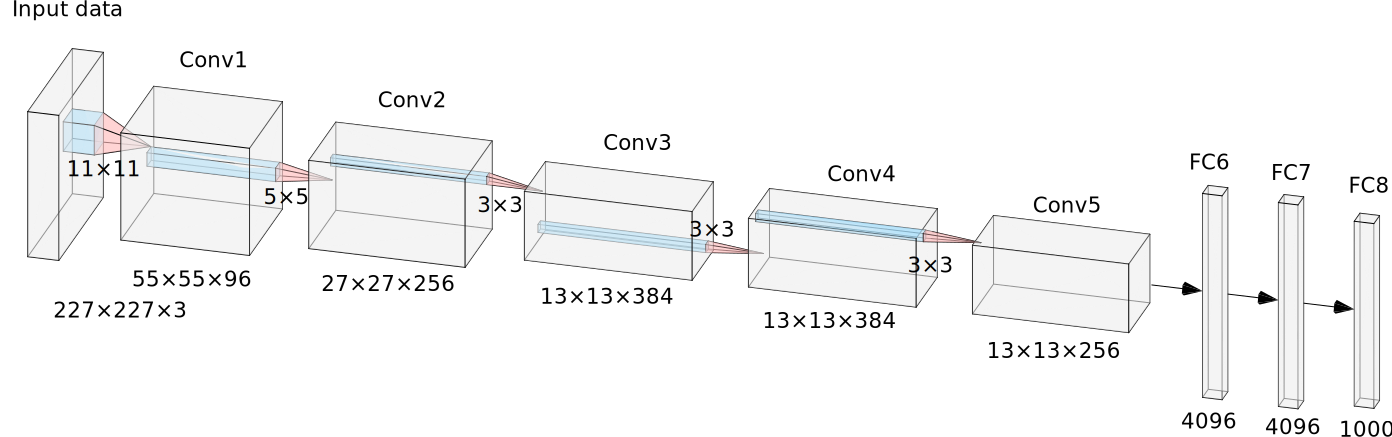
\includegraphics[width=0.5\textwidth]{addestramento-rete-neurale/alexnet.pdf}
        %\caption{Architettura della CNN AlexNet}
        %\label{fig:alexnet}
    \end{figure}
    E la si riaddestra per con un altro  dataset, adeguando i livelli finali:
    \begin{figure}[ht]
        \centering
        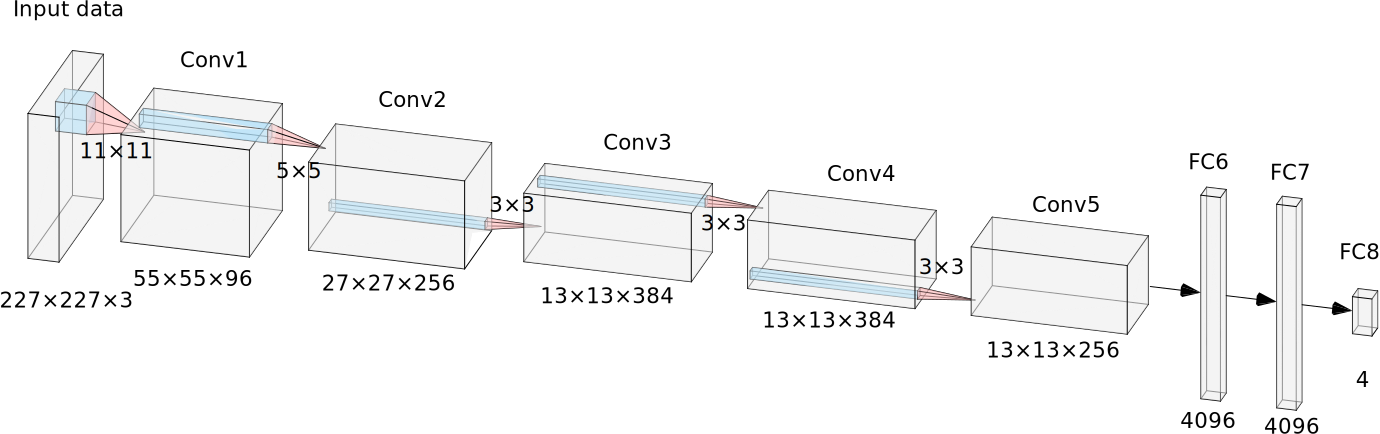
\includegraphics[width=0.5\textwidth]{addestramento-rete-neurale/alexnet-tl.pdf}
        %\caption{Architettura della rete neurale AlexNet adeguata alla classificazione del dataset oggetto di studio}
        %\label{fig:alexnet-tl}
    \end{figure}
\end{frame}

\begin{frame}{Transfer Learning}{Two Round turing}
    Il Two Round turing è una tecnica che effettua due Fine Tuning per l'allenamento della rete, di cui il primo basato su un dataset simile a quello di destazione.
    \begin{figure}[ht]
        \centering
        \includegraphics[width=0.6\textwidth]{transfer-learning/tl_2rt.pdf}
        %\caption[Schema dei due approcci: In giallo il One round turing (1R), in verde il Two round tuning]{Schema dei due approcci: In giallo il One round turing (1R), in verde il Two round tuning. Le frecce piene denotano l'input per l'addestramento, le frecce tratteggiate denotano i flussi di output (modelli addestrati).}
        %\label{fig:tl_2rt}
    \end{figure}
\end{frame}

\section{Preprocessing}
\begin{frame}{Preprocessing}
    Il preprocessing è l'attività che serve a migliorare le immagini, attività incentivata a migliorare i risultati nella fase di addestramento. In particolare si useranno i metodi:
    \begin{itemize}
        \item Ottimizzazione del contrasto (tramite valori hardoced, dinamici e CLAHE)
        \item Correzzione Gamma
    \end{itemize}
\end{frame}

\section{Data augmentation}
\begin{frame}{Data augmentation}
    Partendo da una immagine raster, per esempio rappresentata nel formato tensoriale:
    \begin{figure}[ht]
        \centering
        \tdplotsetmaincoords{75}{20}
        \begin{tikzpicture}[tdplot_main_coords]
            \begin{scope}[canvas is xz plane at y=2,transform shape]
                \node[inner sep=0pt,text=blue,opacity=0.8] (mat1)
                {\(\displaystyle\begin{bmatrix*}[c]
                        f_b(1,1) & f_b(1,2) & \cdots & f_b(1, m) \\ f_b(2,1) & f_b(2,2) & \cdots & f_b(2, m) \\ \vdots & \vdots & & \vdots \\ f_b(n,1) & f_b(n,1) & \cdots & f_b(n,m) \\
                    \end{bmatrix*}\)};
    
                \begin{scope}[on background layer]
                    \fill[blue,opacity=0.2] (mat1.south west) coordinate (blb) -- (mat1.south east) coordinate (brb) -- (mat1.north  east) coordinate (trb) -- (mat1.north  west) coordinate (tlb);
                \end{scope}
            \end{scope}
            %
            \begin{scope}[canvas is xz plane at y=0,transform shape]
                \node[inner sep=0pt,text=green!70!black,opacity=0.8] (mat2) {\(\displaystyle
                    \begin{bmatrix*}[c]
                        f_g(1,1) & f_g(1,2) & \cdots & f_g(1, m) \\ f_g(2,1) & f_g(2,2) & \cdots & f_g(2, m) \\ \vdots & \vdots & & \vdots \\ f_g(n,1) & f_g(n,1) & \cdots & f_g(n,m) \\
                    \end{bmatrix*}\)};
    
                \begin{scope}[on background layer]
                    \fill[green!70!black,opacity=0.2] (mat2.south west) coordinate (blb) -- (mat2.south east) coordinate (brb) -- (mat2.north  east) coordinate (trb) -- (mat2.north  west) coordinate (tlb);
                \end{scope}
            \end{scope}
            %
            \begin{scope}[canvas is xz plane at y=-2,transform shape]
                \node[inner sep=0pt,text=red,opacity=0.8] (mat3) {\(\displaystyle
                    \begin{bmatrix*}[c]
                        f_r(1,1) & f_r(1,2) & \cdots & f_r(1, m) \\ f_r(2,1) & f_r(2,2) & \cdots & f_r(2, m) \\ \vdots & \vdots & & \vdots \\ f_r(n,1) & f_r(n,1) & \cdots & f_r(n,m) \\
                    \end{bmatrix*}\)};
    
                \begin{scope}[on background layer]
                    \fill[red,opacity=0.2]
                    (mat3.south west) coordinate (blb) -- (mat3.south east) coordinate (brb) -- (mat3.north  east) coordinate (trb) -- (mat3.north  west) coordinate (tlb);
                \end{scope}
            \end{scope}
            %\foreach \X in {tl,tr,br}
            %{\draw[thin,orange] (\X f) -- (\X b);}
            %\begin{scope}[on background layer]
            % \draw[thin,orange] (blf) -- (blb);
            %\end{scope}
            \node[left] at (mat2.west) {\(f(x,y,k)=\quad \quad\)};
        \end{tikzpicture}
    \end{figure}
    A cui vengono applicate semplici trasformazioni geometriche come:
    \begin{multicols}{2}
    \begin{itemize}
        \item Riflessione
        \item Ridimensionamento
        \item Rotazione
        \item Traslazione 
    \end{itemize}
    \end{multicols}
\end{frame}

\begin{frame}{Data augmentation}{Discrete cousene transform}
    In aggiunta ai suddetti metodi, si può lavorare attraverso la DCT a metodi per modificare i valori delle frequenze dell'immagine.

    \begin{figure}[ht]
        \centering
        
\includegraphics[width=1\textwidth]{data-augmentation/dct-trasformazione.pdf}
        %\caption{Architettura di una trasfromazione via DCT}
        %\label{fig:dct-schema}
    \end{figure}
    Dove:
    \[\operatorname{DCTimage} ( x , y ) = \alpha( x ) \alpha (y) \sum _ { \mathclap{(p , q) = (1,1)} } ^ { \mathclap{(n,m)} }  \operatorname { Image } ( p , q ) \cos \left(\frac { \pi p  (x-1) } { 2 n }  \right) \cos \left(\frac { \pi q  (y-1) } { 2 m }  \right) \]
    Per ogni \((x,y) \in [0..n]\times [0...m]\), dove \(n,m\) rappresentano la dimensione dell'immagine. Similmente la DCT tipo III o IDCT è definita come:
    \[\operatorname{IDCTimage} ( x , y ) = \sum _ { \mathclap{(p , q) = (1,1) }} ^ {  \mathclap{(n,m) }} \alpha( p ) \alpha (q) \operatorname { DCTimage } ( p , q ) \cos \left(\frac {  \pi p  (x-1) } { 2 n }  \right) \cos \left(\frac { \pi q  (y-1) } { 2 m }  \right) \]
\end{frame}

\section{Risultati}
\begin{frame}{Risultati}
    \begin{table}[H]
        \centering
        \begin{tabular}{l|cc|cc}
                                         & \multicolumn{2}{c|}{1R}                                                   & \multicolumn{2}{c}{2R}                                                   \\
                                         & (1) & (2) & (1) & (2) \\ \midrule
        Semplice DA                      & 95.4\%                            & 100\%                                & 97.5\%                            & 100\%                                \\
        Filtro Contrasto Semplice        & 96.2\%                            & 100\%                                & 96.2\%                            & 100\%                                \\
        Filtro Contrasto con media e STD & 89.6\%                            & 91.7\%                               & 92.9\%                            & 100\%                                \\
        CLAHE                            & 63.7\%                            & 45.8\%                               &                                   &                                      \\
        Correzione Gamma                 & 95.0\%                            & 100\%                                &                                   &                                      \\
        Correzione Gamma e CLAHE         & 46.0\%                            & 0\%                                  &                                   &                                      \\
        Noise                            & 96.7\%                            & 100\%                                & 95.4\%                            & 95.0\%                               \\
        DCT e Noise                      & 94.6\%                            & 100\%                                & 93.8\%                            & 100\%                             
        \end{tabular}
        %\caption[Specchio riassuntivo delle performance singole dei vari metodi analizzati]{Specchio riassuntivo delle performance singole dei vari metodi analizzati, (1): Divisione corretta nelle 4 classi, (2): Riconoscimento dei frame Informative}
        %\label{tab:specchio-single}
    \end{table}
\end{frame}
\begin{frame}[c]{ }
    \centering
    Grazie!
    \end{frame}

\end{document}